\chapter{Sparse coding}
%\thispagestyle{empty}

\Todo{better intro}
The Cambridge Advanced Learner defines a code as ``..a system of numbers,
letters or signals which is used to represent something in a shorter or more
convenient form'' A sparse code is a sparse vector of coefficients that is used
to linear combine a small selection of atoms from a dictionary. Sparse code have
their origin in neural science and machine learning. Olshausen and Field in 1996
\cite{Olshausen1996}

Consider $X \in \mathbb{R}^{m\times n}$  as a matrix with $n$ columns each
column $x_{i}$ representing a signal described by a single vector of
signal length $m$. The dictionary $D\in\mathbb{R}^{m \times p}$ is another
matrix with $p$ columns where each column represents an atom signal with the
same dimension as a single signal $x_{i}$ from $X$. The vector $\alpha$ is
linear combination of a few non orthonormal atoms from $D$ that is close to the
signal $X$. The problem is not well-posed because there is more than one
solution. 

%Sparse coding is the 
\begin{align}
x \approx D\alpha\notag\\
\underbrace{\begin{pmatrix} x_1 \\ x_2 \\ \vdots \\ x_n \end{pmatrix}}_{signal} \approx \underbrace{\begin{pmatrix} d_1  d_2 \cdots d_n \end{pmatrix}}_{\textrm{dictionary atoms}}
\underbrace{\begin{pmatrix} \alpha_1 \\ 0 \\ \vdots \\ \alpha_n \end{pmatrix}}_{\textrm{sparse vector}}
\end{align}

The solution to this problem is a least-squares solve under-determined linear
system we want the sparsest solution. We try to keep coefficient vector $\alpha$
sparse.
\begin{align}
\min_{\alpha\in\mathbb{R}^{p}} \underbrace{\lVert x - D\alpha \rVert^{2}_{2}}_{reconstruction} \label{eq:problem}
\end{align}


\section{Regularization}
To achieve the spare solution we add a constraint to the problem. 
%.. over-fitting .. Such a constraint is the regularization.
\begin{align}
\min_{\alpha\in\mathbb{R}^{p}} \lVert x - D\alpha \rVert^{2}_{2} + \underbrace{\psi(\alpha)}_{regularization}
\end{align}

The sparsity is measured with the $\ell_0$ pseudo-norm in the form
of $\lVert\alpha\rVert_{0}$. The regularization with the $\ell_0$-norm makes the
initial problem \ref{eq:problem} NP-hard. To get the ideal solution it is
necessary to test every combination of atoms. But this does not imply that there
is no way to efficiently find a solution that is good enough to to keep $\alpha$
sparse. There exist several greedy algorithms that can solve the problem in a
not perfect but good enough way. Another approach would be to use $\ell_1$ or
$\ell_2$ as a convex relaxation of $\ell_0$-norm.

It can be demonstrated that the $\ell_1$-norm is equivalent to the $\ell_0$-norm .....
\Todo{image/description of different regularizations}

In the last 15 years several sparse coding algorithms have been proposed. Some
that solve the initial $\ell_0$ regularized problem greedily, like
the (orthogonal)-matching-pursuit, and others which modified the problem to
become convex/linear. These primary derive from the numerical domain in the form
of large linear system solvers with few optimization constraints. The
LARS-Lasso, Ridge regressio, basis pursuit, FOCUSS.


%copy
% Following Tao et al., where it was shown that the L1 norm is equivalent to the L0 norm, 
%leads one to solve an easier problem. Finding the candidate with the smallest L1 norm can be expressed relatively
%easily as a linear program, for which efficient solution methods already exist. These solution methods have been refined over the past few years yielding enormous gain

\begin{figure}
\centering
%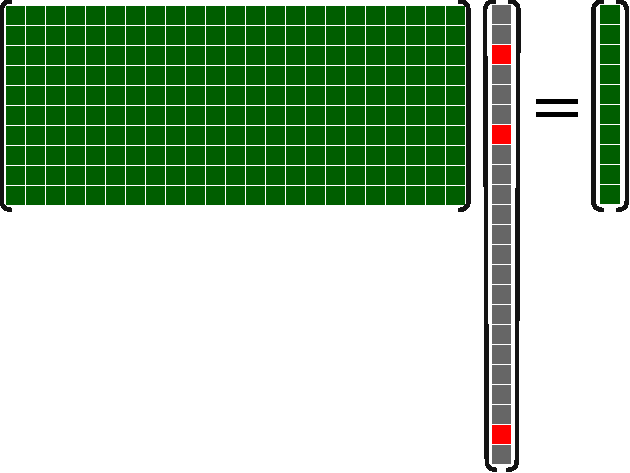
\includegraphics[width = 0.66\textwidth]{images/Da_x.pdf} % Or .pdf
\caption{Sparse Coding}
\label{fig:da_x}
\end{figure}






\section{$\ell_0$ regularization with greedy algorithms}
These algorithms calculate a coefficient vector $\alpha$ which is an
greedy solution of the following NP-hard problem

\begin{align}
\min_{\alpha\in\mathbb{R}^{p}}  \lVert x - D\alpha \rVert^{2}_{2} \textrm{ s.t. } \lVert \alpha \rVert_{0} \leq L
\end{align}
respectivly
\begin{align}
\min_{\alpha\in\mathbb{R}^{p}}   \lVert \alpha \rVert_{0}   \textrm{ s.t. } \lVert x - D\alpha \rVert^{2}_{2} \leq \epsilon
\end{align}
\cite{Mallat1993}

\subsection{Matching-Pursuit}
\label{sec:mp}

The \prettyref{alg:mp} starts with the coefficent vector $\alpha$ set to
zero. Then find the atom in the dictionary with the best reduction of the
error. This is done by selecting the coefficient that has the maximum
correlation with the residual. Repeat this step $L$ times or until the error
$\lVert x - D\alpha \rVert^{2}_{2}$ for the curernt $\alpha$ reaches $\lVert x -
D\alpha \rVert^{2}_{2} \leq \epsilon$ respectifly the residual fullfills $\lVert
r \rVert_2 \leq \epsilon$.


\begin{algorithm}
\caption{Matching Pursuit}
\label{alg:mp}
\begin{algorithmic}[1]
\REQUIRE $x \in \mathbb{R}^m, D \in \mathbb{R}^{m\times p}, L \in \mathbb{N}, \epsilon \in \mathbb{R}$
\STATE $\alpha_0 \gets 0$ (start with zero vector)
\STATE $r_0 \gets x-D\alpha_0 = x$ (residual) 
\WHILE {$\lVert \alpha \rVert_{0} \leq L$ $\lVert r \rVert_2 \leq \epsilon$}
\STATE Select atom with maximum correlation with residual: 
\begin{equation*}
i \gets \argmax_{i=1,...,p} \lvert \left<d_i,r\right> \rvert
\end{equation*}
\STATE update coefficients: 
\begin{align}
a[i]  \gets a[i] + \left<d_i,r\right> \label{eq:mp_update}
\end{align}

\STATE update residual: $r \gets r - \left<d_i,r\right>d_i$

\ENDWHILE
\RETURN $\alpha$
\end{algorithmic}
\end{algorithm}
\subsection{Orthogonal-Matching-Pursuit}
\label{sec:omp}

An improved version of the \prettyref{sec:mp} the the
Orthogonal-Matching-Pursuit \prettyref{alg:omp} was presented by
in\cite{Pati1993}. Rather than just updating the coefficent of $\alpha$ that is
currently selected \prettyref{eq:mp_update} the algorithm re-evaluates all
coefficent in the current active set $S$  \prettyref{eq:omp_update} $\alpha_S$
by solving a full least-squares solution in every iteration. This improves the
quality of the solution.\cite{OMP} The name Orthogonal-Matching-Pursuit comes
from the fact that the residual $r$ is orthogonal to the previously selected
atoms in $D$ which leads to the effect that every coefficent is only selected
once.


\begin{algorithm}
\caption{Orthogonal Matching Pursuit}
\label{alg:omp}
\begin{algorithmic}[1]
\REQUIRE $x \in \mathbb{R}^m, D \in \mathbb{R}^{m\times p}, L \in \mathbb{N}, \epsilon \in \mathbb{R}$
\STATE $\alpha \gets 0, r \gets x $ (residual) $, A \gets \emptyset$
\FOR {$j = 0$ to $L$}
\STATE Select atom with maximum correlation with residual: 
\begin{equation*}
i \gets \argmax_{i \in A^C} \lvert \left<d_i,r\right> \rvert
\end{equation*}
\STATE update active set: $A \gets A \cup \{i\} $
\STATE update residual: $r \gets \left(I-D_A\left( D_A^T D_A \right)^{-1} D_A^T \right)x$
\STATE update coefficients: 
\begin{align}
a_A \gets \left( D_A^T D_A \right)^{-1} D_A^T x  \label{eq:omp_update}
\end{align}

\ENDFOR
\RETURN $\alpha$
\end{algorithmic}
\end{algorithm}

%\subsection*{Limitations}

All these gready approaches tend to find suitable solutions but because of the
non-convex problem they can get stuck in local minimas. As shown before an
$\ell_1$ regularization version of \ref{eq:problem} also keeps the coefficent
vector $\alpha$ sparse but elimantes the problem of a local minima. The next
section presents algorithms which solve  a $\ell_1$ regularization version of
\ref{eq:problem}.



\section {$\ell_1$ regularization}



The Lasso (least absolute shrinkage and selection operator) is a
regularized version of a least squares solution. The regularized version is
found by adding a constraint that induces the $L_1$-norm of the solution to be
small.\cite{Tibshirani1996}

\begin{align}
\min_{\alpha\in\mathbb{R}^{p}}   \lVert \alpha \rVert_{1}   \textrm{ s.t. } \lVert x - D\alpha \rVert^{2}_{2} \leq \epsilon\label{eq:l1}
\end{align}

The lagrange multiplier version of the regularized problem \ref{eq:l1} is:

\begin{align}
\min_{\alpha\in\mathbb{R}^{p}}  \frac{1}{2} \lVert x - D\alpha \rVert^{2}_{2} + \lambda \lVert \alpha \rVert_{1}
\end{align}

There are several ways to compute the LASSO. .. ...... 

LARS \cite{lars} basis pursuit\cite{BASIS_PURSUIT}  FOCUSS \cite{FOCUSS}

We chose the LARS method as it is the fastest in low dimension or for
high correlation. Both conditions are satisfied in our experiments. \Todo{split
into LAR and LARS-lasso, better illustrate than use complex formulas}


\subsection {LARS-Lasso}
\label{sec:lars}
The LARS-Lasso is a algorithm to solve the LASSO with the help of least
angle regression. as described in \cite{Efron2004}. It is a modified version of
the LAR where variables get removed from the active set when their coefficent
become zero.

\paragraph{Least angle regression}
The main idea of the least angle regression is to start with all coefficent zero
$\alpha = 0$. Find the variable $x_i$ with the maximum correlation with the
residual $r$ and then move linear into the direction of the ordinary least
squares solution until a new variable has a higher correlation with the
residual. 


\begin{align}
\min_{\alpha\in\mathbb{R}^{p}}  \frac{1}{2} \lVert x - D\alpha \rVert^{2}_{2} + \lambda \lVert \alpha \rVert_{1}
\end{align}

\begin{algorithm}
\caption{LARS-lasso}
\begin{algorithmic}[1]
\REQUIRE $x \in \mathbb{R}^m, D =[d_1,...,d_p] \in \mathbb{R}^{m\times p}, L \in \mathbb{N}, \epsilon \in \mathbb{R}$
% xD normalized and centered
\STATE $\alpha \gets 0, \mu_{0} \gets 0, A \gets \emptyset$
\FOR {$j = 0$ to $L$}
\STATE calculate correlations with residual: $c \gets D^t\left( x-\mu_j \right) $
\STATE Select atom with maximum correlation: 
\begin{equation*}
i \gets \argmax_{i \in A^C} \lvert c_i  \rvert % \left<d_i,x-\mu_{j}\right>
\end{equation*}
\STATE maximum correlation: $c_{max} \gets c_i $ %\left<d_a,r\right> $\STATE update active set: $A \gets A \cup \left{i\right} $
\STATE calculate movement into OLS direction:
\STATE signs of the correlations: $s_A \gets  sign\left(c_A\right)$
\STATE $\tilde{D_A} \gets D_A\left(\ldots s_id_i \ldots\right)_{i\in A}$
\STATE $G_A \gets \tilde{D_A}^t\tilde{D_A}$
\STATE calculate angle: $A_A \gets \left( 1_A^{-1} G_A^{-1} 1_A \right)^{-\frac{1}{2}}$
\STATE apply weights: $w_A \gets A_AG_A^{-1}1_A$
\STATE equiangular direction: $u_A \gets D_Aw_A$
\STATE correlation between direction and variables: $a \gets D_tu_A$
\STATE minimal movement:
\begin{equation*}
\gamma \gets \min_{i\in A^C}^{+} \left\lbrace \frac{c_{max}-c_i }{A_A-a_i }, \frac{c_{max}+c_i }{A_A+a_i } \right\rbrace
%\gamma \gets \min_{i\in A^C}^{+} \left\lbrace \frac{c_{max}-\left< x,d_i \right> }{1-\left< d_a,d_i \right> }, \frac{c_{max}+\left< x,d_i \right> }{1+\left< d_a,d_i \right> } \right\rbrace
\end{equation*}
\STATE drop coefficent from active that change sign: 
\STATE $ \tilde{\gamma} \gets -\alpha/s_A^tw_A  $
\STATE $ i \gets \min_{i\in A}^{+} \left( \tilde{\gamma}_i \right) $
%\STATE $ i \gets \alpha_{i} = 0, i \in A $
\IF {$\tilde{\gamma}_i>0$ and $\tilde{\gamma}_i<\gamma$}
\STATE remove from active set: $ A \gets A \backslash \{i\} $
\STATE update movement: $ \gamma \gets \tilde{\gamma} $  
\ENDIF
%\STATE $ \mu_{j+1} \gets \mu_{j} - \gamma x_i $
\STATE $ \mu_{j+1} \gets \mu_{j} - \gamma u_a $
\STATE $ \alpha \gets \alpha - \gamma s_A^tw_A $

\ENDFOR

\end{algorithmic}
\end{algorithm}

\subsubsection*{Limitations}
The Lasso modified version of the LAR algorithm has the following limitations.
\begin{description}
 \item[Dimension] When the dimension $p$ of the signal $X$ is much higher than
the the dimension $m$ of the dictionary $D$ the algorithm can only select $m$
columns.
  \item[correlation] When the columns of the dictionary are highly correlated
the algorithm selects only one column.
\end{description}

Limitation one is irrelevant for our experiments as the dictionaries are over-complete 
, with respect to the dimension $m$ of signal $X$, and thus satisfy $p\leq n$.

\section{Application and Related Work}

%\begin{description}
\paragraph{noise reduction}
Remove noise from a signal. 
Using the fact that sparse coding is an approximation of signal that loses ...
noise? ... in its encoding process. 
\begin{align*}
y = x + w
\end{align*}

\cite{Elad2006}


\paragraph{in-painting}
fill missing parts by removing rows from the dictionary
Train with the original image
\begin{align*}
x \approx D\alpha\\
x_s \approx D_s\alpha\\
Wx \approx WD\alpha\text{select subset}\\
\end{align*}

\cite{mairal08sparse}

\paragraph{compression} \cite{Murray2006} \cite{Lewicki1999} An example for this
is the compression of facial images by Bryt and Elad \cite{Bryt2008}.

%Task driven dictionaries
\paragraph{classification} Examples for this can be found in
\cite{Mairal2008b} and \cite{Bar2009}.

\paragraph{inverse half-toning} ongoing research by Mairal et al., 2010
\cite{Mairal2010b}

\paragraph{super resolution} \cite{Yang2010} \cite{Wright2008}  
Or the ongoing work by Couzinie-Devy et al., 2010 called digital zooming.

\paragraph{background subtraction} \cite{}

\paragraph{sense spase signals}\cite{Duarte2009}
%\item[noise reduction]
%\item[in-painting]
%\item[classification] \Todo{usage:classification}

%\end{description}





